\section{MCL Algorithm}

% https://www.mathworks.com/help/nav/ref/montecarlolocalization-system-object.html

\begin{frame}{MCL Algorithm}
    
    {\scshape Goal:} localizing the position of the UAV.

    \begin{block}{How does it work?}
        \begin{itemize}
            \item Estimates its position and orientation;
            \item first interaction: uniform distribution;
            \item the later ones gets more precise.
        \end{itemize}
    \end{block}

\end{frame}

% -----------------------------------------------------------------------------

\begin{frame}{MCL Algorithm (State Representation)}
    
    \begin{columns}
        \begin{column}{0.55\textwidth}
            \begin{itemize}
                \item three element vector (\(x, y, \theta\));
                \item initial input;
                \item mean of the highest weighed cluster of particles.
            \end{itemize}
        \end{column}
        \hfill
        \begin{column}{0.35\textwidth}
            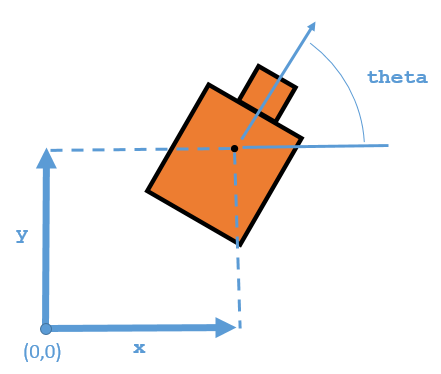
\includegraphics[width=\columnwidth]{figures/robot_pose.png}
        \end{column}
    \end{columns}

\end{frame}

% -----------------------------------------------------------------------------

\begin{frame}{MCL Algorithm (Initialization of Particles)}

    \begin{columns}
        \begin{column}{0.45\textwidth}
            \begin{block}{Global Localization}
                \begin{itemize}
                    \item initial position is unknown;
                    \item particles uniformly distributed;
                    \item less performance.
                \end{itemize}
            \end{block}
        \end{column}
        \hfill
        \begin{column}{0.45\textwidth}
            \begin{block}{Initial pose}
                \begin{itemize}
                    \item initial location is given;
                    \item more particles acummulated at the initial pose;
                    \item more performance.
                \end{itemize}
            \end{block}
        \end{column}
    \end{columns}
    
\end{frame}

% -----------------------------------------------------------------------------

\begin{frame}{MCL Algorithm (Resampling Particles)}

    \begin{itemize}
        \item {\itshape UpdateThreshold:} minimum amount of necessary change in the three element vector.
        \item {\itshape ResamplingInterval:} defines the number of necessary updates for particle resampling.
    \end{itemize}
    
\end{frame}